\documentclass[11pt,a4paper]{article}
\usepackage[T1]{fontenc}
\usepackage[utf8]{inputenc}
\usepackage[a4paper,margin=22mm]{geometry}
\usepackage{microtype}
\usepackage{amsmath,amssymb}
\usepackage{graphicx}
\usepackage{booktabs,array}
\usepackage[table]{xcolor}
\usepackage[numbers,sort&compress]{natbib}
\usepackage[hidelinks]{hyperref}
\usepackage[font=small,labelfont=bf]{caption}
\graphicspath{{../figures/supplementary/}}
\newcommand{\abbrevnote}[1]{\par\vspace{0.25em}{\footnotesize\textbf{Abbreviations:} #1\par}}
\renewcommand{\thefigure}{S\arabic{figure}}
\renewcommand{\thetable}{S\arabic{table}}
\renewcommand{\theequation}{S\arabic{equation}}

\title{Supplementary Information for: A multiscale model connects nanosecond electric pulses with extracellular vesicle population dynamics}
\author{Arash Ghorbannia, Mihir Mantena, Ruben M. L. Colunga-Biancatelli}
\date{}

\begin{document}
\maketitle

\section*{Supplementary Note 1: Layer-specific simulation behavior}

The following figures separate the upstream and downstream behaviors condensed into Fig.~2 of the main manuscript. They are retained as supporting diagnostics because their purpose is to expose model behavior, not to provide independent experimental validation.

\begin{figure}[htbp]
\centering
\includegraphics[width=0.82\textwidth]{supplementary_figure1_temperature.png}
\caption{\textbf{Electrical-dose models give different thermal interpretations.} Temperature-related outputs are shown for the legacy, adiabatic and lumped-retention representations under illustrative conductivity and pulse-train conditions. Curves are simulated from provisional parameters and should not be interpreted as measured temperature.}
\end{figure}

\begin{figure}[htbp]
\centering
\includegraphics[width=0.82\textwidth]{supplementary_figure2_voltage.png}
\caption{\textbf{Pulse width and cell size determine reduced membrane charging.} The first-order electrodynamic model approaches the Schwan-limit voltage more closely for longer pulses and larger cells. Values are simulated and the permeability threshold is a model parameter.}
\end{figure}

\begin{figure}[htbp]
\centering
\includegraphics[width=0.86\textwidth]{supplementary_figure3_ion_transport.png}
\caption{\textbf{Electroporation states generate distinct ionic and bioenergetic trajectories.} Baseline, higher-dose, calcium-limited and slow-recovery simulations are compared for calcium, osmotic, mitochondrial, reactive-oxygen and adenosine-triphosphate states. Curves show model output rather than experimental replicates.}
\end{figure}

\begin{figure}[htbp]
\centering
\includegraphics[width=0.86\textwidth]{supplementary_figure4_repair.png}
\caption{\textbf{Calcium-dependent remodeling separates buffering, cytoskeletal disruption and repair.} Simulated buffered, calpain-inhibited and annexin/lysosome-supported conditions are compared for phosphatidylserine exposure, actin remodeling and resealing.}
\end{figure}

\begin{figure}[htbp]
\centering
\includegraphics[width=0.86\textwidth]{supplementary_figure5_biogenesis.png}
\caption{\textbf{Biogenesis states distinguish secretory and injury-associated particle routes.} Simulations compare Rab/endosomal-sorting limitation, ceramide-favored secretion and injury-associated vesiculation. AB, apoptotic body; EV, extracellular vesicle; MVB, multivesicular body.}
\end{figure}

\begin{figure}[htbp]
\centering
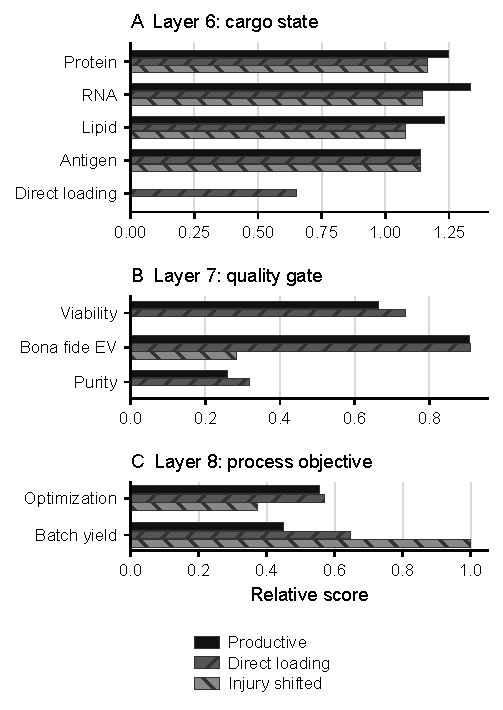
\includegraphics[width=0.78\textwidth]{supplementary_figure6_engineering.pdf}
\caption{\textbf{Downstream product metrics distinguish particle output from product quality.} Simulated cargo, potency, purity, viability and process objectives are shown for secretion-favored, direct-loading and injury-associated conditions. Values are dimensionless model outputs and are not calibrated potency measurements.}
\end{figure}

\clearpage
\section*{Supplementary Note 2: Calibration diagnostics}

\begin{figure}[htbp]
\centering
\includegraphics[width=\textwidth]{supplementary_figure7_fit_error.png}
\caption{\textbf{Residual structure varies with diameter, condition and harvest time.} Signed normalized difference was calculated as $100(\mathrm{model}-\mathrm{experiment})/(\mathrm{model}+\mathrm{experiment})$; the absolute maps show its magnitude. Each cell is an observed diameter band at 0.5, 1 or 3 h. No intermediate times are interpolated. Low-concentration tail bands can have large relative differences because an instrument detection-limit mask was unavailable.}
\end{figure}

\begin{figure}[htbp]
\centering
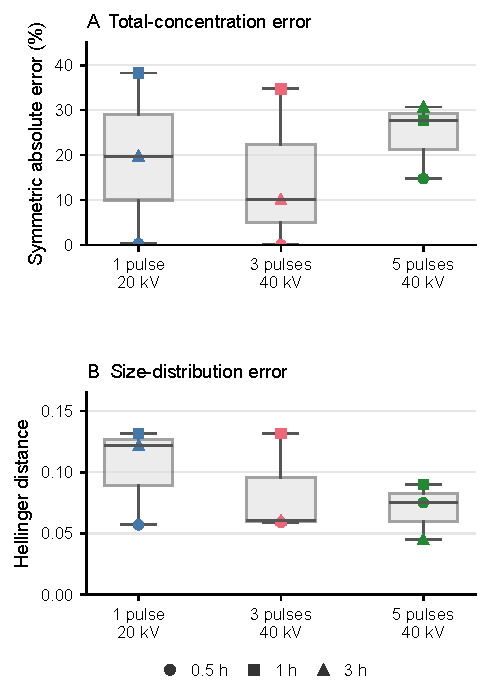
\includegraphics[width=0.72\textwidth]{supplementary_figure8_error_summary.pdf}
\caption{\textbf{Calibration errors differ among pulse-labelled conditions.} a, Symmetric absolute concentration error over 80--380 nm. b, Hellinger distance between normalized size distributions. Each box summarizes three harvest times and does not represent a biological-replicate confidence interval.}
\end{figure}

\clearpage
\section*{Supplementary Note 3: Sensitivity and local-information diagnostics}

\begin{figure}[htbp]
\centering
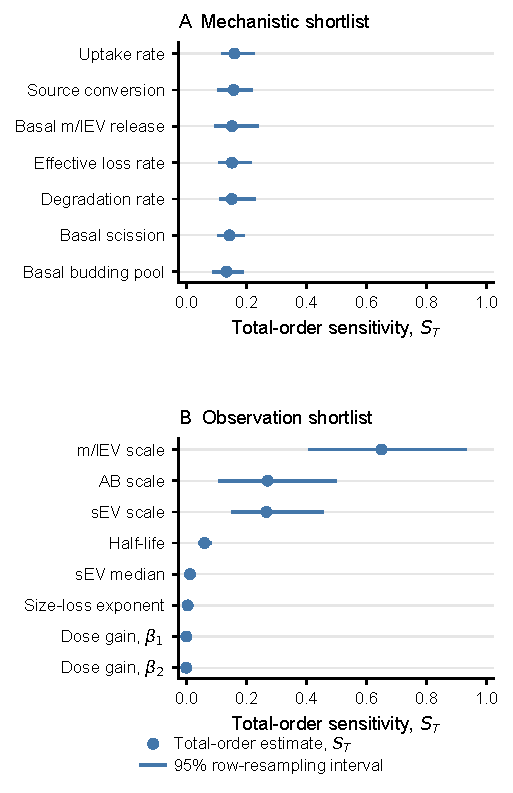
\includegraphics[width=0.78\textwidth]{supplementary_figure9_sobol.pdf}
\caption{\textbf{Conditional total-order estimates remain uncertain for shortlisted parameters.} Points show Jansen total-order estimates from 64 base rows; horizontal intervals show the 2.5th--97.5th percentiles from 200 paired-row resamples. Unselected parameters were fixed. Intervals describe resampling variation and do not establish convergence or biological uncertainty.}
\end{figure}

\begin{figure}[htbp]
\centering
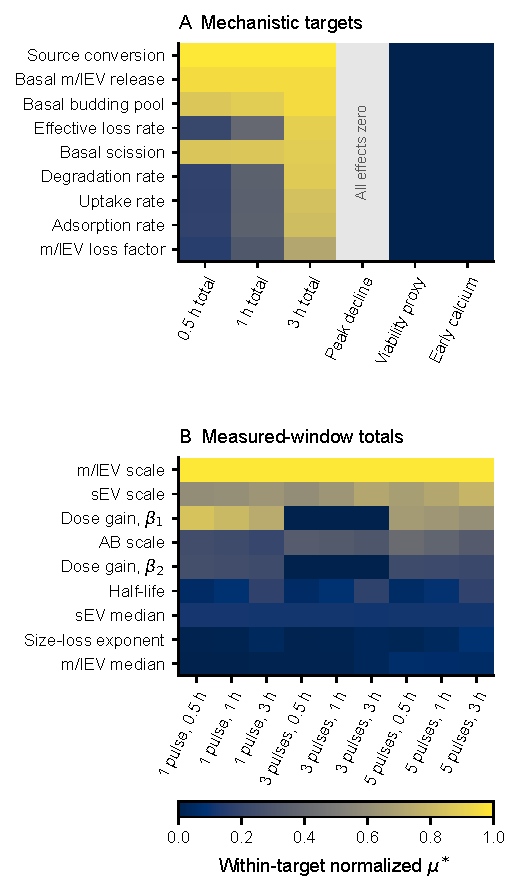
\includegraphics[width=0.8\textwidth]{supplementary_figure10_output_map.pdf}
\caption{\textbf{Screening patterns depend on output and exposure condition.} Colour shows the Morris mean absolute elementary effect divided by its within-target maximum. The normalization supports comparison of patterns within a target, not absolute magnitude across targets. Gray denotes undefined normalization when all computed effects were zero.}
\end{figure}

\begin{figure}[htbp]
\centering
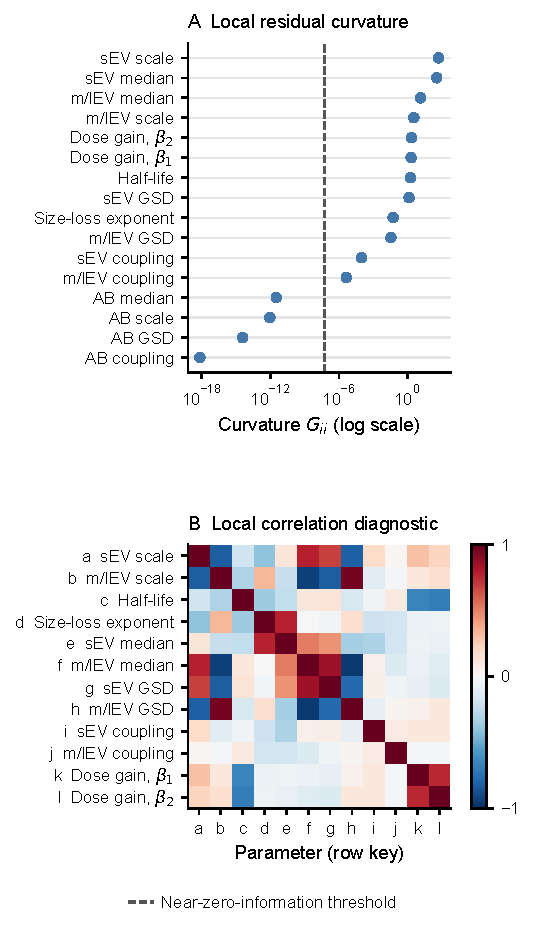
\includegraphics[width=0.78\textwidth]{supplementary_figure11_identifiability.pdf}
\caption{\textbf{The selected fit contains weak and correlated parameter directions.} a, Diagonal of the parameter-scaled residual-curvature matrix; the dashed line is the near-zero-information threshold. b, Normalized entries of its truncated generalized inverse after parameters below the threshold were omitted. These are local geometric diagnostics, not posterior correlations or confidence intervals.}
\end{figure}

\begin{figure}[htbp]
\centering
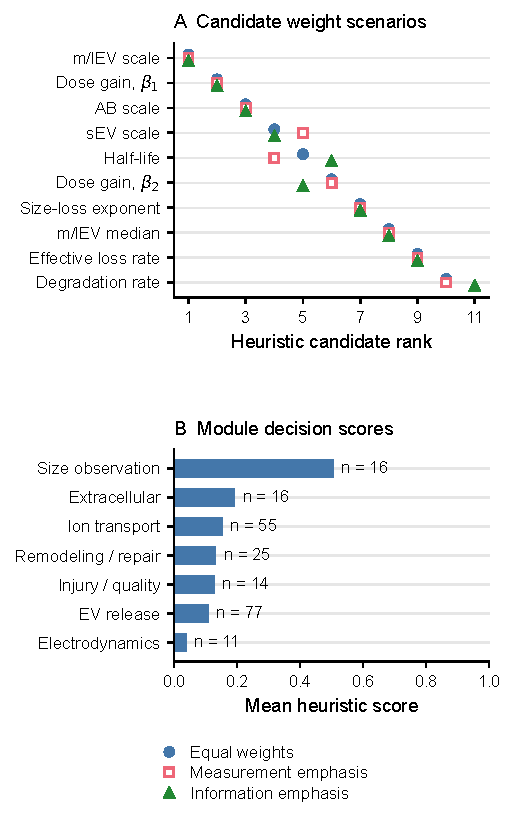
\includegraphics[width=0.78\textwidth]{supplementary_figure12_priorities.pdf}
\caption{\textbf{Measurement-priority scores are stable only for the leading candidate.} a, Ten highest equal-weight candidates under equal, measurement-emphasis and information-emphasis weights. b, Module-average decision scores; $n$ is the number of screened parameters. Feasibility and measurability were assigned heuristically, so the scores are decision aids rather than optimized study designs.}
\end{figure}

\clearpage
\section*{Supplementary Note 4: Extended model specification}

The paired evidence and computational tables, governing-equation scaffold and complete variable glossary from the preceding manuscript have been moved here to keep the main article focused on findings. They document the intended model interfaces and the evidential status of reduced equations. Entries marked as hypotheses or assumptions are not presented as experimentally established mechanisms.

\setlength{\tabcolsep}{3pt}
\subsection*{Appendix organization and model-curation strategy}
The appendix is organized as paired biological and computational tables for each modeling layer. The biological tables document the experimental and mechanistic rationale for including each submodule. The computational tables document candidate mathematical representations, variables, inputs, outputs, and parameterization strategies. Evidence confidence is determined by literature review using the following working categories: established, supported, hypothesized, or model assumption. Table pairs are referenced locally in each module subsection so that biological claims and candidate model forms can be traced back to their evidence and implementation tables.

% ============================================================
\subsection*{Pulse Delivery, Exposure Geometry, and Dosimetry}
% ============================================================

Pulse delivery, exposure geometry, and dosimetry define the engineered exposure that initiates electro-exocytosis. In this layer, the pulse waveform denotes the externally imposed electric-field history, including pulse amplitude, duration, number, polarity, and repetition rate. Early nsPEF studies show that these variables set the transition from plasma-membrane poration to intracellular Ca$^{2+}$ mobilization, PS exposure, and cell-fate responses \cite{beebe2003nanosecond,vernier2003calcium,pakhomov2007membrane,semenov2013primary}. Exposure geometry denotes the physical arrangement of electrodes, chamber, cuvette, culture format, or flow path that converts a programmed voltage waveform into the electric field experienced by the sample. Because cells may receive different effective exposures depending on electrode gap, edge effects, medium conductivity, cell density, sample volume, and position within the device, geometry is central to reproducibility \cite{joshi2000electroporation,kotnik2019membrane,baker2024numerical}. A nominal pulse protocol is therefore not sufficient unless the exposure configuration, field uniformity, and measurement method are also defined \cite{rems2013cell,leveque2017measurement}. The biological/process evidence for these exposure variables is summarized in Table~\ref{T_A1_bio_dosimetry}, and the corresponding computational abstractions are listed in Table~\ref{T_A2_comp_dosimetry}.

For the present compartmental modeling framework, the spatial field calculation should be treated as an upstream dosimetry and calibration step rather than as a spatially resolved biological state. Device settings and exposure geometry can be collapsed into lumped descriptors such as an effective field amplitude, a cumulative pulse-dose index, a heating constraint or temperature history, an exposure-uniformity factor, and the recovery or harvest interval. These descriptors define controllable engineering inputs and batch-to-batch exposure conditions for the downstream ODE modules, while avoiding the need to track chamber position as a dynamic state variable. This separation is also biologically important: energy deposition and Joule heating must be monitored so that field-driven signaling can be distinguished from thermal artifacts, and the recovery interval must be specified because EV yield, cargo composition, and viability are measured over minutes to hours after pulsing rather than at the instant of exposure. Recent nsPEF spheroid work explicitly links pulse width, repetition rate, buffer conductivity, absorbed energy density, and measured temperature rise, showing that high-conductivity media and compressed pulse trains can produce substantially different thermal histories even when nominal pulse amplitudes are similar \cite{orlacchio2023effects}. Related cancer-ablation studies emphasize the same practical distinction between absorbed electrical dose and heat retained during the treatment interval \cite{gudvangen2022electroporation}. Figure~\ref{fig:dosimetry_schematic} summarizes this interface between device-level pulse delivery and reduced model inputs.

We therefore use a tiered dosimetry strategy in which increasingly detailed pulse-energy models can be selected according to the available calibration data. The simplest baseline preserves a legacy absorbed-energy descriptor,
\begin{equation}
u_{\mathrm{legacy}}=\sigma E_{\mathrm{peak}}^{2}t_pN ,
\end{equation}
where $\sigma$ is the medium conductivity, $E_{\mathrm{peak}}$ is the nominal peak electric field, $t_p$ is pulse width, and $N$ is pulse number. This expression is useful as a transparent dose index and maintains continuity with early exploratory simulations, but it does not distinguish square, bipolar, or exponentially decaying waveforms and treats geometry correction only as a coarse scalar.

A waveform-aware Joule model retains the same physical skeleton but weights the pulse by the normalized squared waveform integral,
\begin{align}
\chi_w &= \frac{1}{t_p}\int_0^{t_p}\left(\frac{E(t)}{E_{\mathrm{peak}}}\right)^2dt,\\
u_J &= \sigma E_{\mathrm{peak}}^{2}t_pN\chi_w\langle g_E^2\rangle,\\
\Delta T_{\mathrm{ad}} &= \frac{u_J}{C_v}.
\end{align}
Here $\chi_w$ captures waveform shape, $\langle g_E^2\rangle$ represents the geometry-averaged squared-field factor, and $C_v$ is the volumetric heat capacity. This adiabatic estimate is intentionally conservative: it represents the temperature rise that would occur if deposited energy remained locally retained. It is appropriate for ranking protocols by electrical energy deposition, but it should not be interpreted as a measured sample temperature when heat diffusion, convection, electrode heat exchange, or long inter-pulse intervals are relevant.

When temperature history is needed, the adiabatic estimate can be coupled to a reduced thermal-retention model,
\begin{equation}
\Delta T_{\mathrm{end}}=\eta\Delta T_{\mathrm{ad}}
\frac{\tau_{\mathrm{loss}}}{T_{\mathrm{train}}}
\left(1-e^{-T_{\mathrm{train}}/\tau_{\mathrm{loss}}}\right),
\end{equation}
where $T_{\mathrm{train}}\approx N/f_{\mathrm{rep}}$ is the pulse-train duration, $\tau_{\mathrm{loss}}$ is an empirical thermal relaxation time, and $\eta$ is a setup-dependent retention factor. This reduced form is not a substitute for finite-element thermal modeling, but it captures the main experimental observation that identical absorbed energy can lead to different end-of-train temperature rises when pulse repetition rate, train duration, buffer conductivity, and exposure geometry differ \cite{orlacchio2023effects,gudvangen2022electroporation}. Because temperature can itself modulate membrane fluidity, permeabilization thresholds, and cell fate, thermal terms should be reported as independent dosimetry outputs rather than folded silently into an electrical dose scalar \cite{kanduser2008temperature,song2011synergistic,song2017thermal,yan2021synergistic,pakhomova2013two}.

\begin{figure*}[t]
    \centering
    \includegraphics[width=0.95\textwidth]{supplementary_figure13_dosimetry_schematic.png}
    \caption{\textbf{Conceptual interface for pulse delivery, exposure geometry, and dosimetry.} The programmed nsPEF waveform and physical exposure configuration determine the actual sample exposure. In a reduced compartmental framework, spatial field information is used for upstream calibration and then summarized as lumped descriptors such as effective field amplitude, cumulative pulse dose, heating constraint, exposure-uniformity factor, and recovery interval. These descriptors provide reproducible inputs to downstream biological ODE modules without requiring a spatially resolved core model.}
    \abbrevnote{nsPEF, nanosecond pulsed electric field; ODE, ordinary differential equation.}
    \label{fig:dosimetry_schematic}
\end{figure*}

\begin{table*}[t]
\footnotesize\sf
\centering
\caption{Biological evidence table for pulse delivery, exposure geometry, and dosimetry.\label{T_A1_bio_dosimetry}}
\rowcolors{2}{gray!10}{white}
\begin{tabular}{p{2.4cm} p{3.0cm} p{3.8cm} p{2.7cm} p{3.4cm}}
\toprule
\textbf{Submodule} & \textbf{Biological/process phenomenon} & \textbf{Evidence to curate} & \textbf{Relevance to EV engineering} & \textbf{Confidence} \\
\midrule
Pulse waveform & nsPEF duration, amplitude, number, repetition rate & Parameter-response studies across pulse width, field strength, repetition, and pulse number & Defines controllable input space for EV yield and cargo modulation & Established \cite{beebe2003nanosecond,vernier2003calcium,pakhomov2007membrane,semenov2013primary,orlacchio2023effects} \\
Exposure geometry & Electrode/chamber/cuvette/flow geometry & Field uniformity, edge effects, cell density, medium conductivity & Controls reproducibility and batch exposure & Supported; implementation remains lumped \cite{joshi2000electroporation,kotnik2019membrane,baker2024numerical,leveque2017measurement,orlacchio2023effects} \\
Energy and heating & Joule heating and thermal artifact risk & Absorbed energy density, waveform energy factor, temperature traces, duty-cycle and repetition-rate effects & Separates bioelectric effects from heat-induced stress & Supported; setup-specific calibration needed \cite{orlacchio2023effects,gudvangen2022electroporation,kanduser2008temperature,song2011synergistic,song2017thermal} \\
Recovery interval & Post-pulse harvest window & EV release and repair kinetics over seconds to hours & Determines when yield, cargo, and viability are measured & Supported\cite{silkunas2026peculiarities,szwedowicz2026reversible,bhattacharya2022calcium,muratori2017activation,williams2023annexin} \\
Scale-up mode & Static versus flow-through treatment & Flow exposure, residence time, process monitoring, and sterility constraints & Connects mechanism to manufacturing implementation & Hypothesized\cite{liu2026microfluidic,bakute2024microphysiological,garcia2016microfluidic,bonakdar2017microfluidic,li2015electroporation} \\
\bottomrule
\end{tabular}
\rowcolors{2}{}{}
\abbrevnote{nsPEF, nanosecond pulsed electric field; EV, extracellular vesicle.}
\end{table*}

\begin{table*}[t]
\footnotesize\sf
\centering
\caption{Computational framework table for pulse delivery, exposure geometry, and dosimetry.\label{T_A2_comp_dosimetry}}
\rowcolors{2}{gray!10}{white}
\begin{tabular}{p{2.6cm} p{3.0cm} p{4.6cm} p{2.8cm} p{2.8cm}}
\toprule
\textbf{Submodule} & \textbf{Model form} & \textbf{Representative relation} & \textbf{Inputs} & \textbf{Outputs} \\
\midrule
Pulse input & External forcing function \cite{beebe2003nanosecond,vernier2003calcium,pakhomov2007membrane,semenov2013primary} & $E(t)=E_0u(t;t_p,N,f)$ & amplitude, width, number, repetition & $E(t)$ \\
Dose metric & Selectable absorbed-energy model \cite{orlacchio2023effects,gudvangen2022electroporation} & $u=\sigma E_{\mathrm{peak}}^2t_pN\chi_w\langle g_E^2\rangle$ & pulse train, conductivity, waveform, geometry & energy density, dose index \\
Field distribution & Laplace/quasi-static field model \cite{joshi2000electroporation,kotnik2019membrane,baker2024numerical,leveque2017measurement} & $\nabla\cdot(\sigma\nabla\phi)=0$, $E=-\nabla\phi$ & chamber geometry, conductivity & local $E(\mathbf{x},t)$ \\
Thermal constraint & Adiabatic or lumped heat-loss model \cite{orlacchio2023effects,gudvangen2022electroporation,kanduser2008temperature,song2011synergistic,song2017thermal} & $\Delta T_{\mathrm{end}}=F_{\mathrm{ret}}\Delta T_{\mathrm{ad}}$ & field, medium, cooling, pulse train & $T(t)$, $\Delta T_{\mathrm{end}}$ \\
Flow-through exposure & Residence-time model \cite{liu2026microfluidic,garcia2016microfluidic,bonakdar2017microfluidic,li2015electroporation} & $D_E(\mathbf{x})=\int_{\tau} E(\mathbf{x}(t))^2dt$ & flow rate, chamber field & exposure distribution \\
\bottomrule
\end{tabular}
\rowcolors{2}{}{}
\abbrevnote{EV, extracellular vesicle.}
\end{table*}
% ============================================================
\subsection*{Plasma Membrane and Organelle Electrodynamics}
% ============================================================

A central goal of the framework is to connect nsPEF exposure to downstream Ca$^{2+}$-dependent EV release and cargo modulation without requiring a complete whole-cell reconstruction. The membrane and organelle-electrodynamics layer therefore serves as the upstream bioelectric perturbation module. The applied pulse induces transient plasma-membrane polarization, electropore formation, increased conductance, and ion-specific permeability, all of which have been observed or modeled in single-cell electroporation studies \cite{kotnik2000analytical,krassowska2007modeling,pakhomov2007long}. Short pulses can also couple to intracellular membranes, supporting reduced organelle-voltage terms for ER, mitochondrial, endosomal, and MVB-related perturbation \cite{vernier2003calcium,semenov2013primary,beebe2012transient,baker2024numerical}. These outputs provide the primary interface between nsPEF exposure and downstream Ca$^{2+}$, repair, exocytosis, EV-biogenesis, and cargo-sorting modules.

Computational electroporation literature clarifies how much of this upstream module can remain reduced while still being mechanistically anchored. Molecular dynamics studies show field-driven water defects progressing into hydrophilic pores on nanosecond time scales, with pore formation, water-channel growth, voltage removal, and resealing all occurring as distinct processes \cite{tieleman2004molecular,tarek2005membrane}. Vesicle electromechanics adds the continuum constraint that breakdown voltage depends on membrane tension, area expansivity, and lipid composition \cite{needham1989electro}. Together, these papers support the present choice to keep pore nucleation, pore-radius/tension effects, permeability, and resealing as separable calibrated states rather than one binary permeabilization switch. Table~\ref{T_A3_bio_electrodynamics} summarizes the biological electrodynamics evidence, and Table~\ref{T_A4_comp_electrodynamics} lists the reduced computational forms used for this layer.

The current implementation uses a reduced electrodynamics ladder rather than a full spatial pore-kinetic simulation. Plasma-membrane polarization is represented by a Schwan-style limiting voltage scaled by the effective field, cell radius, and a cell-state membrane modifier, with a first-order charging correction for finite pulse width:
\[
\begin{aligned}
\Delta V_m^{\infty} &= f_sE_{\mathrm{eff}}aM_m, \\
\Delta V_m(t_p) &= \Delta V_m^{\infty}
\left(1-\exp[-t_p/\tau_m]\right).
\end{aligned}
\]
where $f_s$ is the Schwan geometry factor, $E_{\mathrm{eff}}$ is the geometry-corrected electric field, $a$ is the configurable cell radius, $M_m$ is the membrane-state modifier, $t_p$ is pulse width, and $\tau_m$ is an effective membrane charging time \cite{kotnik2000analytical,joshi2000electroporation,kotnik2019membrane}. This formulation resolves the previous fixed-radius placeholder by making $\Delta V_m$ explicitly cell-size dependent; larger cells reach higher induced membrane voltages at the same field, while very short pulses may terminate before the membrane reaches its Schwan limit.

Electroporation is then represented by reduced permeability and pore-density closures:
\[
\begin{aligned}
P_m &= \left[1+\exp[-s(\Delta V_m-V_{\mathrm{th}})]\right]^{-1}, \\
N_p &= N_{\max}
\frac{\Delta V_m^n}{V_{1/2}^n+\Delta V_m^n}.
\end{aligned}
\]
These terms are phenomenological surrogates for voltage-dependent pore creation, pore growth, conductance, and resealing models \cite{vasilkoski2006absolute,krassowska2007modeling}. Patch-clamp studies provide direct calibration targets because nsPEF-induced conductance can persist for minutes and recover in a cell-type-dependent manner \cite{pakhomov2007membrane,pakhomov2007long,nesin2012cell}. The reduced pore-density variable should therefore be interpreted as an effective permeability state, not an absolute physical pore count, until it is calibrated against conductance, dye uptake, ion flux, or recovery data. Organelle perturbation is currently represented by configurable fractions of the plasma-membrane voltage, $\Delta V_o=\alpha_o\Delta V_m$ for ER, mitochondria, and MVB/endosomal membranes. This preserves an explicit route from nsPEF exposure to intracellular membrane stress while marking the organelle layer as calibration-dependent until multi-shell, geometry-resolved, or organelle-specific simulations are incorporated \cite{semenov2013primary,beebe2012transient,baker2024numerical}. The same pore state also feeds the lipid-remodeling layer because experiments and MD simulations connect nanosecond-pulse nanopores with voltage-driven phosphatidylserine translocation \cite{vernier2006nanoporeJACS,vernier2006nanoporePhysBio}.

\begin{table*}[t]
\footnotesize\sf
\centering
\caption{Biological evidence table for plasma membrane and organelle electrodynamics.\label{T_A3_bio_electrodynamics}}
\rowcolors{2}{gray!10}{white}
\begin{tabular}{p{2.4cm} p{3.1cm} p{3.7cm} p{2.8cm} p{4.0cm}}
\toprule
\textbf{Submodule} & \textbf{Biological phenomenon} & \textbf{Evidence to curate} & \textbf{Relevance to EV engineering} & \textbf{Confidence} \\
\midrule
Membrane polarization & Rapid transmembrane-potential rise & Measurements or simulations of $\Delta V_m$ under nsPEF exposure & Determines whether local membrane regions reach electroporation range & Established; reduced Schwan/charging implementation \cite{kotnik2000analytical,joshi2000electroporation,kotnik2019membrane,baker2024numerical} \\
Plasma-membrane nanopores & Transient nanoscale membrane defects & Conductance, dye uptake, ion permeability, recovery kinetics & Creates pathways for Ca$^{2+}$ and other ion entry & Established; pore-density proxy remains phenomenological \cite{pakhomov2007membrane,pakhomov2007long,vasilkoski2006absolute,krassowska2007modeling,kotnik2019membrane} \\
Organelle electroporation & ER, mitochondrial, nuclear, endosomal, and MVB membrane perturbation & Ca$^{2+}$ release, mitochondrial depolarization, intracellular membrane access & Provides route for store release, ROS, and altered MVB/cargo dynamics & Supported; organelle fractions need calibration \cite{vernier2003calcium,semenov2013primary,beebe2012transient,baker2024numerical} \\
Permeability recovery & Conductance decay and resealing & Patch clamp, uptake assays, dye exclusion & Sets duration and magnitude of post-pulse ion flux & Established; kinetics are cell-type dependent \cite{pakhomov2007long,nesin2012cell,pakhomov2007membrane,pakhomova2013two} \\
Isolated EV permeabilization & Direct nsPEF effect on EV membranes & Vesicle integrity, cargo loading, aggregation, marker retention & Defines second mode for post-isolation EV engineering & Hypothesized; not implemented in the current cell-based layer \cite{singh2025electroporation,hood2014maximizing,kooijmans2013electroporation,fuhrmann2015active,didiot2018optimized} \\
\bottomrule
\end{tabular}
\rowcolors{2}{}{}
\abbrevnote{nsPEF, nanosecond pulsed electric field; ER, endoplasmic reticulum; EV, extracellular vesicle; MVB, multivesicular body.}
\end{table*}

\begin{table*}[t]
\footnotesize\sf
\centering
\caption{Computational framework table for plasma membrane and organelle electrodynamics.\label{T_A4_comp_electrodynamics}}
\rowcolors{2}{gray!10}{white}
\begin{tabular}{p{2.6cm} p{3.0cm} p{4.6cm} p{2.8cm} p{2.8cm}}
\toprule
\textbf{Submodule} & \textbf{Model form} & \textbf{Representative relation} & \textbf{Inputs} & \textbf{Outputs} \\
\midrule
Membrane charging & Reduced Schwan/circuit model \cite{kotnik2000analytical,joshi2000electroporation,kotnik2019membrane} & $\Delta V_m=f_sE_{\mathrm{eff}}a(1-e^{-t_p/\tau_m})$ & $E(t)$, geometry, cell radius, membrane state & $\Delta V_m$ \\
Organelle charging & Reduced multi-shell surrogate \cite{semenov2013primary,beebe2012transient,baker2024numerical} & $\Delta V_o=\alpha_o\Delta V_m$ & organelle factors, plasma-membrane voltage & $\Delta V_o$ \\
Pore nucleation & Voltage-dependent permeability proxy \cite{tieleman2004molecular,tarek2005membrane} & $P_m=[1+\exp[-s(\Delta V_m-V_{\mathrm{th}})]]^{-1}$ & $\Delta V_m$, threshold parameters & $P_m$ \\
Pore-radius evolution & Pore-energy or reduced kinetic model \cite{needham1989electro,tarek2005membrane} & $\frac{dr_p}{dt}=F(r_p,\Delta V,\gamma,\sigma)$ & pore energy, tension & $r_p(t)$ \\
Permeability closure & Saturating pore-density closure \cite{smith2004stable,krassowska2007modeling} & $N_p=N_{\max}\Delta V_m^n/(V_{1/2}^n+\Delta V_m^n)$ & pore-density scale, voltage scale, Hill exponent & $N_p$, $P_i$ \\
Isolated EV charging & Vesicle-scale circuit model \cite{singh2025electroporation,hood2014maximizing,kooijmans2013electroporation} & $C_{EV}\frac{d\Delta V_{EV}}{dt}+G_{EV}\Delta V_{EV}=f(E,r_{EV})$ & EV radius, medium conductivity & $P_{EV}(t)$, integrity state \\
\bottomrule
\end{tabular}
\rowcolors{2}{}{}
\abbrevnote{ER, endoplasmic reticulum; EV, extracellular vesicle; MVB, multivesicular body.}
\end{table*}

% ============================================================
\subsection*{Ion Transport, Ca$^{2+}$ Mobilization, ROS, and Bioenergetics}
% ============================================================

The ion-transport and organelle-state module translates nsPEF-induced membrane permeability into intracellular ionic, metabolic, and stress responses. The minimal model treats electropore-mediated Ca$^{2+}$ influx and ER release as source terms in a cytosolic Ca$^{2+}$ balance. More detailed formulations include voltage-gated or leak-channel entry, ER release through IP$_3$ receptors or ryanodine receptors, SERCA-mediated refilling, PMCA and NCX extrusion, mitochondrial uptake and release, ROS generation, ATP dependence, and osmotic recovery. Table~\ref{T_A5_bio_ca_ros} organizes the biological evidence for these submodules, while Table~\ref{T_A6_comp_ca_ros} lists the corresponding reduced flux-balance and organelle-state model forms.

For the current computational framework, this layer is represented as a reduced flux-balance ODE system rather than a full electrodiffusion model. The pore term is treated as a transient extracellular Ca$^{2+}$ source gated by the electrodynamic permeability state. This choice is supported by studies in which nsPEF rapidly elevates cytosolic Ca$^{2+}$ and the response depends on extracellular Ca$^{2+}$, pulse width, and membrane pathway \cite{vernier2003calcium,bagalkot2018membrane,yun2024modulating}. In CHO cells, a 60-ns pulse produced separable external-Ca$^{2+}$ and ER-release thresholds and a critical Ca$^{2+}$ range for amplification, making these data especially useful for tuning reduced Ca$^{2+}$ source terms \cite{semenov2013primary}.

ER mobilization is modeled as an electrically triggered store-release pathway with SERCA refilling, while IP$_3$R/RyR-mediated amplification is retained as a cell-type-specific extension for excitable or store-sensitive cells \cite{semenov2013recruitment,tolstykh2013activation,tolstykh2014pip2,wang2009cardiac,azarov2019excitation}. The computational calcium literature gives useful bounds for that extension: Li and Rinzel reduced a detailed IP$_3$ receptor model to a Hodgkin--Huxley-like form with IP$_3$ regulation, Ca$^{2+}$ activation, and Ca$^{2+}$ inactivation, while Shannon and coworkers used junctional, subsarcolemmal, and bulk compartments with realistic buffering, reversible SR uptake, Na$^+$--Ca$^{2+}$ exchange, and load-dependent release \cite{li1994equations,shannon2004mathematical}. We therefore keep the default ER term compact, but expose channel opening, store content, pump capacity, and exchanger recovery as parameters when cell-type-specific data are available.

Na$^+$, K$^+$, and Cl$^-$ fluxes are included as lumped electropore/channel-mediated perturbations that relax toward baseline and drive an osmotic-stress state. This abstraction is justified by evidence that nsPEF increases leak conductance, depolarizes membrane potential, alters voltage-gated channels, and changes cell volume \cite{pakhomov2007membrane,smith2011transmembrane,burke2017nanosecond,yang2021regulation}. Na$^+$/K$^+$-ATPase sensitivity is retained as a recovery modifier because ATP1A1 silencing attenuates membrane disruption after nanosecond pulses \cite{silkuniene2023silencing}.

Mitochondrial Ca$^{2+}$ uptake/release and depolarization connect cytosolic Ca$^{2+}$ to ROS and ATP availability. nsPEF studies support mitochondrial membrane perturbation and ROS generation, while broader calcium-electroporation data show that Ca$^{2+}$ overload can deplete ATP and shift the cell toward injury \cite{beebe2012transient,napotnik2012mitochondrial,pakhomova2012oxidative,nuccitelli2013reactive,radzeviciute2024calcium,gibot2020calcium}. On the computational side, mitochondrial modules can be scaled from a minimal Ca$^{2+}$-handling block with respiration, ATP synthase, proton leak, adenine nucleotide exchange, uniporter, and Na$^+$--Ca$^{2+}$ exchange \cite{magnus1997minimal}, to a simplified ATP-production model driven by glycolytic and Ca$^{2+}$ inputs \cite{bertram2006simplified}, or to a thermodynamically balanced oxidative-phosphorylation model that conserves mass, charge, and free energy \cite{beard2005biophysical}. ROS is represented with Ca$^{2+}$-, mitochondrial-, osmotic-, and pulse-dependent source terms plus first-order clearance; this reduced form is consistent with models in which ROS production, scavenging, and ROS-sensitive inner-membrane conductance shape mitochondrial potential, NADH, and redox dynamics \cite{cortassa2004mitochondrial,murphy2016mitochondrial,zhang2022crosstalk}. ATP is kept as a normalized production-consumption state coupled to mitochondrial potential, pump activity, repair demand, and oxidative stress.

\begin{equation}
\begin{aligned}
\frac{d[\mathrm{Ca}^{2+}]_i}{dt} &=
J_{\mathrm{Ca,pore}} + J_{\mathrm{VGCC}} + J_{\mathrm{ER,rel}} - J_{\mathrm{SERCA}} \\
&\quad - J_{\mathrm{PMCA}} - J_{\mathrm{NCX}} - J_{\mathrm{mito}} - J_{\mathrm{buffer}} .
\end{aligned}
\end{equation}

\begin{table*}[t]
\footnotesize\sf
\centering
\caption{Biological evidence table for ion transport, Ca$^{2+}$ mobilization, ROS, and bioenergetics.\label{T_A5_bio_ca_ros}}
\rowcolors{2}{gray!10}{white}
\begin{tabular}{p{2.7cm} p{3.4cm} p{4.2cm} p{3.0cm} p{2.0cm}}
\toprule
\textbf{Submodule} & \textbf{Biological phenomenon} & \textbf{Evidence to curate} & \textbf{Relevance to EV engineering} & \textbf{Confidence} \\
\midrule
Electropore Ca$^{2+}$ influx & Rapid extracellular Ca$^{2+}$ entry & Ca$^{2+}$ imaging, chelation, Ca$^{2+}$-free media & Primary trigger for downstream release and repair mechanisms & Established \cite{bagalkot2018membrane,bhattacharya2022calcium,morotomi2014extracellular,yun2024modulating,cantu2021caveolin} \\
ER Ca$^{2+}$ release & Intracellular store mobilization & IP$_3$R/RyR involvement, ER store depletion & Amplifies cytosolic Ca$^{2+}$ transients and fusion signals & Established \cite{semenov2013recruitment,tolstykh2013activation,tolstykh2014pip2,wang2009cardiac,azarov2019excitation} \\
Na$^+$, K$^+$, Cl$^-$ fluxes & Ionic/osmotic perturbation & Membrane-potential recovery, swelling, ionic imbalance & Modulates volume, tension, and repair state & Supported \cite{smith2011transmembrane,burke2017nanosecond,muratori2017activation,silkuniene2023silencing,yang2021regulation} \\
Mitochondrial Ca$^{2+}$ & Uptake/release and depolarization & Mitochondrial Ca$^{2+}$, $\Delta\Psi_m$, mPTP evidence & Links Ca$^{2+}$ to metabolic stress and fate decisions & Supported \cite{beebe2012transient,napotnik2012mitochondrial,murphy2016mitochondrial} \\
ROS generation & Oxidative stress after nsPEF & ROS probes, antioxidant rescue, mitochondrial source evidence & Modifies EV secretion, cargo, and injury transition & Supported \cite{pakhomova2012oxidative,nuccitelli2013reactive,zhang2022crosstalk,lee2019caveolin,wiczew2021molecular} \\
ATP/bioenergetics & Energy availability for pumps and trafficking & ATP depletion, pump recovery, metabolic assays & Controls repair, cargo sorting, and EV-release capacity & Hypothesized \cite{frandsen2012calcium,radzeviciute2024calcium,gibot2020calcium} \\
\bottomrule
\end{tabular}
\rowcolors{2}{}{}
\abbrevnote{EV, extracellular vesicle; ER, endoplasmic reticulum; IP$_3$R, inositol 1,4,5-trisphosphate receptor; RyR, ryanodine receptor; ROS, reactive oxygen species; ATP, adenosine triphosphate; mPTP, mitochondrial permeability transition pore.}
\end{table*}

\begin{table*}[t]
\footnotesize\sf
\centering
\caption{Computational framework table for ion transport, Ca$^{2+}$ mobilization, ROS, and bioenergetics.\label{T_A6_comp_ca_ros}}
\rowcolors{2}{gray!10}{white}
\begin{tabular}{p{2.6cm} p{3.0cm} p{4.6cm} p{2.8cm} p{2.8cm}}
\toprule
\textbf{Submodule} & \textbf{Model form} & \textbf{Representative relation} & \textbf{Inputs} & \textbf{Outputs} \\
\midrule
Pore-mediated Ca$^{2+}$ flux & GHK/Ohmic flux \cite{tieleman2004molecular,tarek2005membrane} & $J_{\mathrm{Ca,pore}}=P_{\mathrm{Ca}}(t)\Phi_{\mathrm{Ca}}(C_e,C_i,V_m)$ & $P_{\mathrm{Ca}}$, gradients, voltage & Ca$^{2+}$ source term \\
ER release & Store-release ODE \cite{li1994equations,shannon2004mathematical} & $J_{\mathrm{ER,rel}}=k_{rel}O_{\mathrm{IP3R/RyR}}(C_i,C_{ER})$ & channel state, store content & ER-to-cytosol flux \\
Pump/exchanger recovery & Saturating fluxes \cite{shannon2004mathematical} & $J_{\mathrm{PMCA}}=V_{max}\frac{C_i^n}{K^n+C_i^n}$ & Ca$^{2+}$, Na$^+$, ATP, voltage & Ca$^{2+}$ clearance \\
Mitochondrial buffering & Coupled uptake/release ODE \cite{magnus1997minimal,bertram2006simplified} & $\frac{dC_m}{dt}=J_{\mathrm{MCU}}-J_{\mathrm{NCLX}}-J_{\mathrm{mPTP}}$ & $C_i$, $\Delta\Psi_m$, ROS & mitochondrial Ca$^{2+}$ state \\
ROS dynamics & Source-clearance ODE \cite{cortassa2004mitochondrial} & $\frac{dR}{dt}=k_{ROS}f(C_m,\Delta\Psi_m)-k_{clear}R$ & mitochondrial state, antioxidants & ROS state variable \\
ATP state & Production-consumption ODE \cite{beard2005biophysical,bertram2006simplified} & $\frac{dA}{dt}=k_{prod}f(\Delta\Psi_m)-k_{use}(J_{pump}+R_{repair})$ & mitochondria, pumps, repair & ATP availability \\
\bottomrule
\end{tabular}
\rowcolors{2}{}{}
\abbrevnote{ER, endoplasmic reticulum; GHK, Goldman-Hodgkin-Katz; PMCA, plasma membrane Ca$^{2+}$ ATPase; MCU, mitochondrial calcium uniporter; NCLX, Na$^+$/Ca$^{2+}$/Li$^+$ exchanger; ROS, reactive oxygen species; ATP, adenosine triphosphate; mPTP, mitochondrial permeability transition pore.}
\end{table*}

% ============================================================
\subsection*{Ca$^{2+}$-Dependent Remodeling and Repair}
% ============================================================

This module connects global and submembrane Ca$^{2+}$ signals to local membrane remodeling and repair. Although cytosolic Ca$^{2+}$ may be represented as a well-mixed compartment in reduced models, electro-exocytosis is likely governed by local Ca$^{2+}$ domains near pores, damaged membrane regions, budding sites, repair complexes, and fusion machinery. Reaction--diffusion theory provides a practical reason to distinguish these domains from the bulk pool: mobile and immobile buffers can confine Ca$^{2+}$ elevations over nanometer-to-submicrometer distances, with local gradients forming on submillisecond time scales near an open channel \cite{naraghi1997linearized}. Ca$^{2+}$-dependent resealing occurs on experimentally measurable time scales, with nano- and microsecond electroporation studies reporting fast and slow repair components that are sensitive to extracellular Ca$^{2+}$ \cite{bhattacharya2022calcium}. Local Ca$^{2+}$ therefore serves not only as an influx variable but also as the organizing signal for lipid asymmetry, cytoskeletal mechanics, curvature, scission, fusion competence, and resealing. The paired evidence and modeling assumptions for these repair and remodeling variables are tabulated in Tables~\ref{T_A7_bio_remodel_repair} and \ref{T_A8_comp_remodel_repair}.

For the current computational framework, this layer is implemented as a reduced Ca$^{2+}$-sensor and repair-state module. The upstream ion-transport state is converted into a submembrane Ca$^{2+}$ microdomain proxy amplified by pore activation and osmotic stress, with buffer strength and shell depth treated as tunable parameters rather than fixed geometry. This choice reflects evidence that ESCRT and repair machinery assemble at damaged membrane domains rather than responding only to bulk cytosolic Ca$^{2+}$ \cite{scheffer2014mechanism,shukla2022vitro}. Annexin recruitment is represented as a Ca$^{2+}$-dependent membrane-binding and curvature-stabilization state because annexin A4/A6/A7 can support membrane constriction, ESCRT-associated repair, and repair-linked vesicle secretion \cite{boye2017annexin,sonder2019annexin,muratori2021role,williams2023annexin}. Molecular and biophysical annexin studies then provide the curvature and lipid-composition rationale for keeping annexin effects separate from generic repair activity \cite{mularski2022interplay,hakamiZanjani2024modulation}.

The lipid-remodeling branch maps local Ca$^{2+}$ to scramblase activation, flippase suppression, and PS externalization. This branch is treated as established because nsPEF activates TMEM16F-dependent PS exposure and blebbing, while newer TIRF studies show delayed, spatially punctate PS externalization after 400-ns pulses \cite{muratori2017activation,silkunas2026peculiarities}. The Vernier studies add a second, faster computationally tractable route: nanopore-facilitated, voltage-driven PS movement can occur along electropore walls and appears experimentally as localized, anode-facing PS externalization after nanosecond pulses \cite{vernier2006nanoporeJACS,vernier2006nanoporePhysBio}. The model therefore keeps an immediate pore/voltage PS term separate from slower Ca$^{2+}$--scramblase dynamics. Chemically controlled TMEM16F vesiculation, lipid-asymmetry loss, and Ca$^{2+}$-regulated flippases provide complementary support for linking Ca$^{2+}$ and PS state to EV-like budding competence \cite{han2019chemically,wang2025loss,segawa2016human}.

The cytoskeletal branch maps local Ca$^{2+}$ to calpain activity, actin disruption, actomyosin tension, and repair-associated shedding. Recent nsPEF actin and swelling studies are especially useful here because Ca$^{2+}$-dependent actin shrinkage and swelling can be tested directly against the model's actin-disruption and osmotic-stress terms \cite{hellwich2026extracellular,pakhomov2014disassembly,rassokhin2014cellular}. Calpain and ezrin-cleavage studies support the protease component, and membrane-repair studies show that calpain can orchestrate annexin-containing microvesicle release \cite{campbell2012structure,roberts2020ca,williams2025calpains}.

Finally, lysosomal repair is represented as a Ca$^{2+}$-triggered vesicle-fusion and membrane-resealing support state. Lysosomal exocytosis, extracellular protease release, sphingolipid-dependent EV biology, lysosomal-channel regulation, and ESCRT-mediated lysosome repair support this reduced repair branch \cite{andrews2014damage,castroGomes2016plasma,verderio2018role,rosato2021two,radulovic2018escrt}. The resulting variables--PS exposure, calpain activity, annexin activity, lysosomal repair, actin state, resealing state, and repair-associated shedding--serve as interpretable coupling terms for medium/large EV budding, membrane recovery, and injury-quality gating.

\begin{table*}[t]
\footnotesize\sf
\centering
\caption{Biological evidence table for Ca$^{2+}$-dependent remodeling and repair.\label{T_A7_bio_remodel_repair}}
\rowcolors{2}{gray!10}{white}
\begin{tabular}{p{2.7cm} p{3.4cm} p{4.2cm} p{3.0cm} p{2.0cm}}
\toprule
\textbf{Submodule} & \textbf{Biological phenomenon} & \textbf{Evidence to curate} & \textbf{Relevance to EV engineering} & \textbf{Confidence} \\
\midrule
Ca$^{2+}$ microdomains & Local Ca$^{2+}$ elevation near pores and membranes & High-speed/local Ca$^{2+}$ imaging, buffer sensitivity & Localizes activation to budding, repair, and fusion sites & Supported \cite{scheffer2014mechanism,shukla2022vitro} \\
Annexin recruitment & Ca$^{2+}$-dependent membrane binding & Annexin translocation and repair studies & Links Ca$^{2+}$ to membrane repair and curvature stabilization & Supported \cite{boye2017annexin,mularski2022interplay,hakamiZanjani2024modulation,muratori2021role,sonder2019annexin} \\
Scramblase/PS exposure & Loss of lipid asymmetry & Annexin V staining, scramblase/flippase studies & Promotes MV-like budding and EV surface phenotype & Established \cite{muratori2017activation,wang2025loss,han2019chemically,silkunas2026peculiarities,segawa2016human} \\
Calpain activation & Ca$^{2+}$-dependent protease activity & Calpain activation/inhibition, cytoskeletal remodeling & Supports blebbing, scission, and membrane remodeling & Supported \cite{williams2025calpains,campbell2012structure,roberts2020ca} \\
Actomyosin remodeling & Tension, contraction, and scission & RhoA/ROCK, myosin, actin perturbation & Determines budding probability and vesicle detachment & Supported \cite{hellwich2026extracellular,pakhomov2014disassembly,rassokhin2014cellular} \\
Lysosomal repair & Ca$^{2+}$-triggered repair-vesicle fusion & LAMP1 exposure, lysosome fusion & Adds membrane and may release vesicle-like material & Supported \cite{andrews2014damage,castroGomes2016plasma,verderio2018role,rosato2021two,radulovic2018escrt} \\
\bottomrule
\end{tabular}
\rowcolors{2}{}{}
\abbrevnote{EV, extracellular vesicle; PS, phosphatidylserine; ESCRT, endosomal sorting complex required for transport.}
\end{table*}

\begin{table*}[t]
\footnotesize\sf
\centering
\caption{Computational framework table for Ca$^{2+}$-dependent remodeling and repair.\label{T_A8_comp_remodel_repair}}
\rowcolors{2}{gray!10}{white}
\begin{tabular}{p{2.6cm} p{3.0cm} p{4.6cm} p{2.8cm} p{2.8cm}}
\toprule
\textbf{Submodule} & \textbf{Model form} & \textbf{Representative relation} & \textbf{Inputs} & \textbf{Outputs} \\
\midrule
Ca$^{2+}$ microdomain & Reaction--diffusion or shell ODE \cite{naraghi1997linearized,shannon2004mathematical} & $\frac{\partial C}{\partial t}=D_{Ca}\nabla^2C+J_{Ca}-R_{buffer}-R_{effector}$ & local flux, diffusion, buffers & $C_{sub}(t)$ \\
Generic Ca$^{2+}$ sensor & Hill activation \cite{naraghi1997linearized,shannon2004mathematical,scheffer2014mechanism} & $A_x=\frac{C_{sub}^n}{K_x^n+C_{sub}^n}$ & local Ca$^{2+}$, sensitivity & activated fraction \\
PS exposure & Activation plus lipid-state ODE \cite{vernier2006nanoporeJACS,vernier2006nanoporePhysBio,muratori2017activation} & $\frac{dPS_{out}}{dt}=k_{scr}A_{scr}(1-PS_{out})-k_{flip}PS_{out}$ & Ca$^{2+}$, scramblase, flippase & PS externalization \\
Calpain/cytoskeleton & Protease activation and substrate loss \cite{campbell2012structure,roberts2020ca,williams2025calpains} & $\frac{dF_{actin}}{dt}=-k_{calp}A_{calp}F_{actin}+k_{poly}$ & Ca$^{2+}$, calpain state & cortical remodeling \\
Membrane resealing & Conductance-recovery ODE \cite{tarek2005membrane,needham1989electro} & $\frac{dG_m}{dt}=-k_{seal}A_{repair}G_m$ & residual conductance, repair activity & resealed membrane state \\
Damaged-domain shedding & Damage-removal rate \cite{needham1989electro} & $R_{shed}=k_{shed}D_m f_{Ca}f_{tension}$ & damaged membrane, Ca$^{2+}$, tension & repair-associated shedding \\
\bottomrule
\end{tabular}
\rowcolors{2}{}{}
\abbrevnote{PS, phosphatidylserine; ODE, ordinary differential equation.}
\end{table*}

% ============================================================
\subsection*{EV Biogenesis and Subtype Release}
% ============================================================

The EV-release module converts nsPEF-induced intracellular and membrane responses into measurable vesicle outputs. It integrates endosomal/MVB-derived small-EV release, plasma-membrane budding of medium/large EVs, and apoptotic body or injury-associated vesiculation. The model should retain mechanistic terms such as exosome and microvesicle internally, but report outputs using EV nomenclature compatible with the level of experimental characterization. The biological release mechanisms are organized in Table~\ref{T_A9_bio_ev_release}, with candidate pool-balance and rate-law implementations listed in Table~\ref{T_A10_comp_ev_release}.

Small-EV production begins with endosome maturation and ILV biogenesis. Recent Rab-conversion studies indicate that Rab5-to-Rab7 transition is not an isolated timing event, but is coordinated with ESCRT-mediated cargo corralling through the Mon1/Ccz1 axis, so maturation and secretory competence should be treated as coupled states rather than as independent switches \cite{ott2025coordination,borchers2023regulatory,solinger2025escrting}. Within maturing endosomes, canonical ESCRT machinery supplies one major ILV route: ESCRT-0 captures ubiquitinated cargo through Hrs/STAM, ESCRT-I/II concentrate cargo and deform the bud neck, and ESCRT-III/Vps4 completes constriction and scission \cite{takahashi2015hrs,wollert2010molecular,pfitzner2020escrt}. However, exosome-biased ILV formation is not exclusively canonical. ALIX-ESCRT-III, ceramide, and tetraspanin-rich membrane domains provide selective alternative routes that can redirect cargo and alter whether MVBs are routed toward secretion or lysosomal degradation \cite{larios2020alix,choezom2022nsmase2,crivelli2022ceramideTransfer,rubinstein2025tetraspanins,villarroyaBeltri2016isgylation}.

Release of those ILVs as extracellular small EVs then depends on trafficking, docking, and fusion at the cell cortex. Rab27, Rab11, and Rab35 families regulate MVB positioning and membrane access, while Munc13-4 provides a Ca$^{2+}$-responsive trafficking and priming branch that helps generate release-competent MVBs \cite{hsu2010rab35,messenger2018munc13,marie2023accessory,izumi2021rab27,tang2026rab27}. The terminal fusion step is mediated by cell-context-dependent SNARE assemblies, with syntaxin-4/SNAP-23/VAMP-7 and VAMP5-based complexes now supported by direct exosome-secretion studies, and with synaptotagmin-7-like Ca$^{2+}$ sensing providing a plausible fusion-pore stabilization mechanism under strong submembrane Ca$^{2+}$ signals \cite{liu2023snare,matsui2023vamp5,woo2017munc13,courtney2023synaptotagmin7}. In parallel, outward budding of medium/large EVs is supported by ARF-, RhoA/ROCK-, phosphatidylserine-, and actomyosin-dependent membrane remodeling, whereas apoptotic bodies arise from caspase-linked ROCK1 activation and repetitive bleb fragmentation during higher-injury states \cite{pang2025arf,dai2019rhoa,menck2017nsmaseMicrovesicles,teixeira2020rock1,ozdemir2021rock1,sakamaki2025mprip}. These mechanistic branches justify treating subtype release as a competition between secretory MVB fate, plasma-membrane budding competence, and apoptotic disassembly rather than as one generic EV-rate variable.

\begin{table*}[t]
\footnotesize\sf
\centering
\caption{Biological evidence table for EV biogenesis and subtype release.\label{T_A9_bio_ev_release}}
\rowcolors{2}{gray!10}{white}
\begin{tabular}{p{2.7cm} p{3.4cm} p{4.2cm} p{3.0cm} p{2.0cm}}
\toprule
\textbf{Submodule} & \textbf{Biological phenomenon} & \textbf{Evidence to curate} & \textbf{Relevance to EV engineering} & \textbf{Confidence} \\
\midrule
Endosome/MVB maturation & Early-to-late endosome and MVB formation & Rab5/Rab7, endosome maturation, ILV evidence & Defines small-EV-producing compartment pool & Established \cite{ott2025coordination,borchers2023regulatory,solinger2025escrting} \\
ESCRT-dependent ILV formation & Cargo sorting and ILV biogenesis & ESCRT, ALIX, TSG101 perturbation & Generates exosome-enriched precursors & Established \cite{takahashi2015hrs,wollert2010molecular,pfitzner2020escrt,larios2020alix} \\
ESCRT-independent ILV formation & Ceramide/tetraspanin/lipid-domain sorting & nSMase2, ceramide, CD63/CD81/CD9 evidence & Alternative small-EV biogenesis route & Supported \cite{choezom2022nsmase2,crivelli2022ceramideTransfer,rubinstein2025tetraspanins} \\
MVB trafficking/docking & Rab-dependent transport to plasma membrane & Rab27A/B, Rab11, Rab35 evidence & Controls release-ready MVB pool & Established \cite{hsu2010rab35,messenger2018munc13,izumi2021rab27,tang2026rab27,marie2023accessory} \\
MVB fusion & SNARE-mediated fusion with plasma membrane & SNARE and Ca$^{2+}$-sensitive fusion evidence & Converts ILVs into secreted small EVs & Supported \cite{liu2023snare,matsui2023vamp5,woo2017munc13,courtney2023synaptotagmin7} \\
Plasma membrane budding & MV-like outward budding & ARF6/RhoA/PS/cytoskeleton studies & Produces medium/large EV precursors & Supported \cite{pang2025arf,dai2019rhoa,menck2017nsmaseMicrovesicles} \\
Apoptotic body formation & Blebbing and fragmentation & Caspase/ROCK1/apoptosis evidence & Captures high-dose or injury-associated vesicles & Established \cite{teixeira2020rock1,ozdemir2021rock1,sakamaki2025mprip} \\
\bottomrule
\end{tabular}
\rowcolors{2}{}{}
\abbrevnote{EV, extracellular vesicle; MVB, multivesicular body; ILV, intraluminal vesicle; ESCRT, endosomal sorting complex required for transport.}
\end{table*}

\begin{table*}[t]
\footnotesize\sf
\centering
\caption{Computational framework table for EV biogenesis and subtype release.\label{T_A10_comp_ev_release}}
\rowcolors{2}{gray!10}{white}
\begin{tabular}{p{2.6cm} p{3.0cm} p{4.6cm} p{2.8cm} p{2.8cm}}
\toprule
\textbf{Submodule} & \textbf{Model form} & \textbf{Representative relation} & \textbf{Inputs} & \textbf{Outputs} \\
\midrule
MVB pool & Compartmental pool balance \cite{huotari2011endosome,ott2025coordination,borchers2023regulatory,solinger2025escrting} & $\frac{dM}{dt}=k_{mat}E_{endo}-k_{dock}M-k_{deg}M$ & endosome pool, maturation & MVB number \\
ILV loading & Production-rate law \cite{takahashi2015hrs,wollert2010molecular,pfitzner2020escrt,larios2020alix,choezom2022nsmase2,crivelli2022ceramideTransfer} & $\frac{dI}{dt}=k_{ILV}f_{ESCRT}M-k_{release}I$ & ESCRT/ceramide state, MVB pool & ILV load \\
MVB docking & Trafficking/docking ODE \cite{hsu2010rab35,messenger2018munc13,izumi2021rab27,tang2026rab27,marie2023accessory} & $\frac{dM_d}{dt}=k_{dock}f_{Rab}M-k_{fus}M_d$ & Rab activity, actin barrier & docked MVB pool \\
Small-EV release & Ca$^{2+}$-sensitive fusion rate \cite{liu2023snare,matsui2023vamp5,woo2017munc13,courtney2023synaptotagmin7} & $R_{sEV}=k_{fus}f_{Ca}(C_{sub})M_d$ & docked MVBs, Ca$^{2+}$, SNARE & small-EV release rate \\
Budding-site formation & Budding pool ODE \cite{pang2025arf,dai2019rhoa,menck2017nsmaseMicrovesicles} & $\frac{dB_{m/lEV}}{dt}=k_{bud}f_{PS}f_{tension}-k_{scission}B_{m/lEV}$ & PS, curvature, tension & budding precursor pool \\
Medium/large EV release & Scission-rate law \cite{pang2025arf,dai2019rhoa,menck2017nsmaseMicrovesicles,williams2025calpains} & $R_{m/lEV}=k_{scission}f_{actomyosin}B_{m/lEV}$ & calpain, ROCK, actomyosin & medium/large EV rate \\
Apoptotic vesicle release & Injury-state weighted rate \cite{teixeira2020rock1,ozdemir2021rock1,sakamaki2025mprip,cappe2023systematic} & $R_{AB}=k_{AB}F_{apop}$ & apoptotic fraction, blebbing rate & apoptotic-body release \\
\bottomrule
\end{tabular}
\rowcolors{2}{}{}
\abbrevnote{MVB, multivesicular body; ILV, intraluminal vesicle; ESCRT, endosomal sorting complex required for transport; sEV, small extracellular vesicle; m/lEV, medium/large extracellular vesicle; AB, apoptotic body.}
\end{table*}

For the current computational framework, this layer is implemented as a reduced pool-balance model with explicit MVB, ILV, docked-MVB, budding-precursor, and apoptotic-commitment states. Endosome maturation is represented as a Rab-conversion-supported source term for a secretory MVB pool, ILV loading is split into ESCRT-dependent and ceramide/tetraspanin-assisted branches, and MVB fate is biased between secretion and lysosomal loss by an acidification-sensitive routing term \cite{ott2025coordination,choezom2022nsmase2,villarroyaBeltri2016isgylation}. Small-EV release is then written as a Ca$^{2+}$- and SNARE-sensitive fusion flux from the docked MVB pool, while medium/large EV release is represented as a phosphatidylserine-, calpain-, and actomyosin-weighted budding/scission process. Apoptotic-body release is modeled separately as a damage- and blebbing-weighted branch so that injury-associated vesiculation is not conflated with productive secretory EV release \cite{liu2023snare,messenger2018munc13,pang2025arf,teixeira2020rock1}. This reduced formulation matches the current code implementation while preserving a direct path for later replacement with cell-type-specific Rab, SNARE, lipid, or apoptosis submodels as quantitative data become available.

% Inter-layer extension connecting mechanistic release pathways to
% size-resolved extracellular measurements. Kept in a separate file to
% minimize merge conflicts with the actively edited main manuscript.
\subsection*{State-Conditioned EV Size--Composition and Observation Bridge}

The release states above specify biological routes, whereas particle-sizing assays report operational diameter classes. These descriptions should remain distinct because endosomal, plasma-membrane, and apoptotic pathways can generate overlapping size ranges, and diameter alone does not establish vesicle origin \cite{welsh2024minimal}. We therefore introduce an inter-layer bridge rather than redefining the existing sEV, m/lEV, and AB states. A biological mode $q$ denotes ESCRT-enriched MVB/ILV release, ceramide/tetraspanin-enriched MVB/ILV release, plasma-membrane shedding or repair-associated release, or apoptotic fragmentation. The first two modes sum to the existing $R_{sEV}$ output, the plasma-membrane mode contributes to $R_{m/lEV}$, and the apoptotic mode contributes to $R_{AB}$. This separation is consistent with evidence that activation can differentially regulate distinct nanosized populations released by CD4$^+$ T cells \cite{vanDerVlist2012activation}.

Let $\mathbf{x}(t)$ denote the upstream cell-state vector, $d$ vesicle diameter, and $\mathbf{c}$ the composition vector. The joint product kernel for biological mode $q$ is factorized as
\begin{equation*}
K_q(d,\mathbf{c}\mid\mathbf{x})
=f_q\!\left(d\mid\boldsymbol{\theta}_q[\mathbf{x}]\right)
g_q(\mathbf{c}\mid d,\mathbf{x}),
\end{equation*}
where $f_q$ is a nonnegative birth-size distribution and $g_q$ represents conditional cargo allocation. Positive right-skewed distributions are appropriate starting points. For MVB-derived small EVs, a dynamic-scaling distribution derived from membrane-domain growth and ILV budding provides a directly implementable candidate; its tail exponent was sensitive to signaling perturbation \cite{paulaitis2018dynamic}. More detailed ESCRT/cargo-crowding membrane models can constrain plausible ILV sizes and coupling signs but introduce unobserved mechanical parameters that are unlikely to be identifiable from sparse longitudinal particle counts \cite{liese2020protein}. Broad lognormal or gamma distributions are therefore retained as reduced alternatives for plasma-membrane and apoptotic modes. Their baseline median and geometric standard deviation should be cell- and assay-specific priors rather than universal subtype constants.

State dependence can be introduced parsimoniously through distribution parameters,
\begin{equation*}
\log d_{50,q}(t)=\alpha_q+
\boldsymbol{\beta}_q^{\mathsf{T}}
\left[\mathbf{z}_q(t)-\mathbf{z}_{q,0}\right],
\end{equation*}
where $\mathbf{z}_q$ contains only pathway-matched states. Candidate inputs include ESCRT and ceramide/secretory routing for MVB modes; PS exposure, calpain, actomyosin, membrane tension, and repair shedding for plasma-membrane release; and damage, apoptosis, and blebbing for the apoptotic mode. The nested null case $\boldsymbol{\beta}_q=\mathbf{0}$ changes pathway mixture weights while retaining fixed within-pathway size distributions.

For true-diameter bin $b=[d_b^-,d_b^+]$, the per-cell birth source and extracellular stock are
\begin{align*}
S_{qb}(t)
&=R_q(t)\int_{d_b^-}^{d_b^+}
f_q\!\left(d\mid\boldsymbol{\theta}_q[\mathbf{x}(t)]\right)\,dd,\\
\frac{dN_{qb}}{dt}
&=N_{\mathrm{cells}}S_{qb}(t)
-k_{\mathrm{loss},q}(d_b)N_{qb}
+\sum_{b'}T_{bb'}N_{qb'}.
\end{align*}
This sectional population balance can use many numerical bins while retaining few shared parameters. It also preserves cohort history: particles remain at their emitted diameter unless an explicit aggregation or fragmentation term $T_{bb'}$ transfers them. Initially, a common effective loss rate and $T_{bb'}=0$ provide the most identifiable model.

Cargo is linked jointly to pathway, state, and size rather than determined by diameter alone. A reduced geometric capacity relation is
\begin{equation*}
\mathrm{E}[C_j\mid d,q,\mathbf{x}]
=a_{jq}(\mathbf{x})d^2+b_{jq}(\mathbf{x})d^3,
\end{equation*}
where the $d^2$ and $d^3$ terms represent membrane-associated and luminal capacity, respectively \cite{zendrini2022surface}. The coefficients retain pathway- and state-dependent sorting, and low-copy cargo can be represented by stochastic occupancy. Single-vesicle measurements showing selective changes in EV size, membrane order, and cargo after Rab27a or CD63 perturbation support this conditional rather than deterministic representation \cite{vonLersner2024multiparametric}.

Finally, biological stocks are mapped to an observed size bin $b$ in assay run $r$ through
\begin{equation*}
\widehat{y}_{rb}(t)=B_{rb}
+\sum_{\ell}H_{rb\ell}\eta_{r\ell}
\frac{\sum_qN_{q\ell}(t)}{V_r},
\end{equation*}
where $H_{rb\ell}$ represents true-to-measured diameter error and rebinning, $\eta_{r\ell}$ represents size-dependent recovery, $B_{rb}$ is background, and $V_r$ is sample volume. This observation operator is required because different single-particle methods can report materially different size distributions and concentrations for the same EV preparation \cite{vanDerPol2014particle,welsh2024minimal}. Instrument-response parameters should be constrained by calibration particles, instrument settings, and orthogonal characterization rather than inferred freely with the biological kernel.

For sparse longitudinal data, calibration should begin with literature- or sham-informed fixed kernels, dynamic pathway mixture weights, and a common extracellular loss term. A state-to-size coefficient should be retained only if it improves prediction for held-out pulse conditions; size-dependent loss should then be tested separately. Particle counts alone cannot identify pathway-specific cargo coefficients, which require marker-resolved or molecular measurements.


% ============================================================
\subsection*{Cargo Sorting, EV Composition, and Potency}
% ============================================================

The cargo module represents the major conceptual expansion from EV-release modeling to EV-engineering modeling. nsPEF may alter EV composition through Ca$^{2+}$-dependent trafficking, stress-responsive transcription and translation, lipid remodeling, ESCRT/tetraspanin/ceramide pathways, RNA-binding proteins, and injury-state contamination. Therefore, EV output should be represented as a multi-dimensional product state rather than as total particle number alone. Table~\ref{T_A11_bio_cargo} separates the biological cargo-sorting evidence, and Table~\ref{T_A12_comp_cargo} specifies the computational cargo, composition, potency, and direct-loading model options.

\begin{table*}[t]
\footnotesize\sf
\centering
\caption{Biological evidence table for cargo sorting, EV composition, and potency.\label{T_A11_bio_cargo}}
\rowcolors{2}{gray!10}{white}
\begin{tabular}{p{2.7cm} p{3.4cm} p{4.2cm} p{3.0cm} p{2.0cm}}
\toprule
\textbf{Submodule} & \textbf{Biological phenomenon} & \textbf{Evidence to curate} & \textbf{Relevance to EV engineering} & \textbf{Confidence} \\
\midrule
Protein sorting & Ubiquitin/ESCRT/tetraspanin-dependent protein enrichment & ALIX, TSG101, CD63/CD81/CD9, antigen enrichment & Determines therapeutic or immunogenic protein cargo & Established \cite{jeppesen2019reassessment,kugeratski2021quantitative,takahashi2015hrs,larios2020alix,rubinstein2025tetraspanins} \\
RNA sorting & RNA-binding protein-mediated miRNA/mRNA loading & hnRNPA2B1, SYNCRIP, YBX1, motif-based sorting & Enables nucleic-acid cargo modulation & Supported \cite{shurtleff2016ybox,liu2021selective,santangelo2016syncrip} \\
Lipid sorting & Ceramide, cholesterol, sphingolipid, PE/PS enrichment & Lipidomics, nSMase2, tetraspanin domains & Controls EV stability, curvature, uptake, immunologic function & Established \cite{skotland2023lipids,choezom2022nsmase2,crivelli2022ceramideTransfer,rubinstein2025tetraspanins} \\
Stress-responsive cargo & ROS, hypoxia, inflammatory, apoptotic cargo changes & proteomics/lipidomics/RNA-seq after nsPEF & Distinguishes programmed cargo modulation from debris & Supported \cite{pakhomova2012oxidative,cappe2023systematic,muratori2017activation} \\
Antigen enrichment & Tumor antigen expression and EV loading & MAGE and other antigen studies & Supports vaccine-oriented EV engineering & Supported \cite{szlasa2024mage,kumar2022tumour} \\
Functional potency & Recipient-cell response & uptake, cargo delivery, immune activation, repair assays & Connects cargo state to biological activity & Hypothesized \cite{hagey2023cellular,tkach2017qualitative,fuhrmann2015active} \\
\bottomrule
\end{tabular}
\rowcolors{2}{}{}
\abbrevnote{EV, extracellular vesicle; ESCRT, endosomal sorting complex required for transport; ALIX, ALG-2-interacting protein X; TSG101, tumor susceptibility gene 101; miRNA, microRNA; mRNA, messenger RNA; PE, phosphatidylethanolamine; PS, phosphatidylserine; RNA-seq, RNA sequencing.}
\end{table*}

\begin{table*}[t]
\footnotesize\sf
\centering
\caption{Computational framework table for cargo sorting, EV composition, and potency.\label{T_A12_comp_cargo}}
\rowcolors{2}{gray!10}{white}
\begin{tabular}{p{2.6cm} p{3.0cm} p{4.6cm} p{2.8cm} p{2.8cm}}
\toprule
\textbf{Submodule} & \textbf{Model form} & \textbf{Representative relation} & \textbf{Inputs} & \textbf{Outputs} \\
\midrule
Subtype-weighted cargo & Weighted output model \cite{jeppesen2019reassessment,kugeratski2021quantitative,cappe2023systematic} & $Cargo_j=w_{j,sEV}R_{sEV}+w_{j,m/lEV}R_{m/lEV}+w_{j,AB}R_{AB}$ & subtype rates, cargo weights & cargo abundance \\
Stress-modulated sorting & Rate law \cite{shurtleff2016ybox,liu2021selective,santangelo2016syncrip,pakhomova2012oxidative} & $\frac{dCargo_j}{dt}=k_{sort,j}f_{stress}f_{Ca}f_{ESCRT}-k_{loss,j}Cargo_j$ & Ca$^{2+}$, ROS, ESCRT, stress & cargo state \\
Antigen enrichment & Transcription/sorting coupling \cite{szlasa2024mage,kumar2022tumour} & $\frac{dA_g}{dt}=k_{expr}f_{stress}-k_{deg}A_g-k_{sort}A_g$ & stress, antigen expression & antigen cargo \\
Lipid composition & Composition-state ODE \cite{skotland2023lipids,choezom2022nsmase2,crivelli2022ceramideTransfer} & $\frac{dL_j}{dt}=k_{syn,j}f_{stress}-k_{sort,j}L_j$ & lipid metabolism, EV subtype & lipid cargo class \\
Potency mapping & Empirical or mechanistic response model \cite{hagey2023cellular,tkach2017qualitative,fuhrmann2015active} & $Potency=F(Cargo,Subtype,Dose)$ & cargo vector, recipient assay & functional potency \\
Direct EV loading & Permeability-diffusion model \cite{kooijmans2013electroporation,hood2014maximizing,fuhrmann2015active,didiot2018optimized} & $\frac{dC_{load}}{dt}=P_{EV}(t)A_{EV}(C_{ext}-C_{EV})-k_{leak}C_{EV}$ & EV permeability, cargo gradient & loaded cargo \\
\bottomrule
\end{tabular}
\rowcolors{2}{}{}
\abbrevnote{EV, extracellular vesicle; ESCRT, endosomal sorting complex required for transport; ALIX, ALG-2-interacting protein X; sEV, small extracellular vesicle; m/lEV, medium/large extracellular vesicle; AB, apoptotic body.}
\end{table*}


The implemented Layer 6 module now follows the table structure explicitly. It computes a subtype-weighted cargo state from small-EV, medium/large-EV, and apoptotic-body outputs; separates protein, RNA, lipid, antigen, and direct-loading terms; and maps the resulting cargo vector to a saturating potency score. This keeps the implementation aligned with evidence that EV subtypes carry distinct protein compositions \cite{jeppesen2019reassessment,kugeratski2021quantitative}, that RNA sorting can be mediated by RNA-binding proteins such as YBX1 and SYNCRIP \cite{shurtleff2016ybox,liu2021selective,santangelo2016syncrip}, that lipid composition and ceramide biology shape EV state \cite{skotland2023lipids}, and that direct EV loading can be represented separately from endogenous cargo sorting \cite{fuhrmann2015active,didiot2018optimized}.

% ============================================================
\subsection*{Injury, Debris, and Quality Gate}
% ============================================================

The injury-quality module defines whether nsPEF exposure produces reversible EV engineering, stress-associated release, apoptosis, necrosis, or contaminating debris. This layer is essential because increased particle number is not necessarily equivalent to increased useful EV production. The quality gate separates bona fide EV output from apoptotic bodies, damaged organellar fragments, protein aggregates, and other co-isolated materials. Table~\ref{T_A13_bio_quality_gate} summarizes the biological and QC evidence for this distinction, while Table~\ref{T_A14_comp_quality_gate} defines the damage, fate-transition, mixture, and constrained-optimization model forms.

\begin{table*}[t]
\footnotesize\sf
\centering
\caption{Biological evidence table for injury, debris, and quality gating.\label{T_A13_bio_quality_gate}}
\rowcolors{2}{gray!10}{white}
\begin{tabular}{p{2.7cm} p{3.4cm} p{4.2cm} p{3.0cm} p{2.0cm}}
\toprule
\textbf{Submodule} & \textbf{Biological phenomenon} & \textbf{Evidence to curate} & \textbf{Relevance to EV engineering} & \textbf{Confidence} \\
\midrule
Viability preservation & Reversible response versus cell death & viability, membrane recovery, clonogenic/metabolic assays & Defines acceptable EV-production window & Established \cite{pakhomova2013two,beebe2012transient,bhattacharya2022calcium} \\
Mitochondrial injury & Depolarization, mPTP, cytochrome c & $\Delta\Psi_m$, cytochrome c, ROS & Separates stress signaling from organellar contamination & Supported \cite{beebe2012transient,napotnik2012mitochondrial,pakhomova2012oxidative} \\
Apoptosis & Caspase activation and apoptotic blebbing & caspase, annexin V/PI, ROCK1 blebbing & Determines apoptotic-body contribution & Established \cite{pakhomova2013two,teixeira2020rock1,cappe2023systematic} \\
Necrosis/lysis & Irreversible membrane failure & LDH release, PI uptake, debris microscopy & Indicates unacceptable product contamination & Established \cite{pakhomova2013two,cappe2023systematic} \\
Non-EV contaminants & Protein aggregates, organelle fragments, apoptotic bodies & calnexin, cytochrome c, albumin/lipoprotein markers & Defines purity and interpretability of EV readouts & Established \cite{webber2013pure,brennan2020comparison,cappe2023systematic,welsh2024minimal} \\
Quality-control marker panel & Positive and negative EV markers & CD63/CD81/CD9, TSG101/ALIX/syntenin, negative markers & Connects model to MISEV-style QC & Established \cite{welsh2024minimal,jeppesen2019reassessment,kugeratski2021quantitative} \\
\bottomrule
\end{tabular}
\rowcolors{2}{}{}
\abbrevnote{EV, extracellular vesicle; mPTP, mitochondrial permeability transition pore; PI, propidium iodide; QC, quality control; MISEV, Minimal Information for Studies of Extracellular Vesicles.}
\end{table*}

\begin{table*}[t]
\footnotesize\sf
\centering
\caption{Computational framework table for injury, debris, and quality gating.\label{T_A14_comp_quality_gate}}
\rowcolors{2}{gray!10}{white}
\begin{tabular}{p{2.6cm} p{3.0cm} p{4.6cm} p{2.8cm} p{2.8cm}}
\toprule
\textbf{Submodule} & \textbf{Model form} & \textbf{Representative relation} & \textbf{Inputs} & \textbf{Outputs} \\
\midrule
Damage accumulation & Damage-state ODE \cite{pakhomova2012oxidative,bhattacharya2022calcium,albeck2008modeling} & $\frac{dD}{dt}=k_{inj}G_m+k_{ROS}ROS-k_{repair}A_{repair}D$ & conductance, ROS, repair & damage burden \\
Fate transition & Hybrid state rule \cite{albeck2008modeling,bentele2004mathematical,pakhomova2013two} & $F_{apop}=H(D-D^*)$ or $\frac{dF_{apop}}{dt}=k_{apop}H(D-D^*)$ & damage, ATP, mitochondria & viable/stressed/apoptotic fractions \\
Necrotic transition & Threshold rule \cite{pakhomova2013two,cappe2023systematic} & $F_{nec}=H(D-D_{nec}^*)H(A_{ATP}^*-ATP)$ & damage, ATP, membrane failure & necrotic fraction \\
Measured particles & Mixture model \cite{cappe2023systematic,webber2013pure,brennan2020comparison} & $N_{meas}=N_{EV}+N_{AB}+N_{debris}+N_{agg}$ & release rates, injury state & measured particle count \\
Purity score & Ratio or classifier \cite{webber2013pure,brennan2020comparison,welsh2024minimal} & $Q_{EV}=\frac{N_{bona\ fide\ EV}}{N_{meas}}$ & marker panel, debris state & EV quality score \\
Acceptable window & Constrained optimization \cite{orlacchio2023effects,gudvangen2022electroporation,welsh2024minimal} & maximize $Y_{EV}$ subject to $Q_{EV}>Q^*$ and $Viability>V^*$ & dose, cell state, harvest & operating region \\
\bottomrule
\end{tabular}
\rowcolors{2}{}{}
\abbrevnote{EV, extracellular vesicle; AB, apoptotic body; ATP, adenosine triphosphate; ROS, reactive oxygen species; QC, quality control.}
\end{table*}


The implemented Layer 7 module expands the previous binary quality proxy into a mixture-aware gate. Damage is mapped to stressed-viable, apoptotic, and necrotic fractions using threshold-like Hill terms inspired by systems models of cell-death switching \cite{albeck2008modeling,bentele2004mathematical}. The measured particle pool is then decomposed into bona fide EVs, apoptotic bodies, debris, and aggregate-like contaminants, which makes the purity score sensitive to both injury state and non-EV co-isolates. This structure matches EV-composition and isolation cautions from apoptotic/necroptotic EV studies and MISEV-style purity guidance \cite{cappe2023systematic,webber2013pure,brennan2020comparison,welsh2024minimal}.

% ============================================================
\subsection*{Manufacturing, Isolation, and Quality-Control Interface}
% ============================================================

The manufacturing module links cell-level mechanisms to translational EV production. It represents harvest timing, cell number, culture format, isolation recovery, marker-based QC, purity, batch variability, and flow-through scalability. This module is intentionally placed after biological release and quality gating because manufacturing success depends on both biological production and downstream process recovery. Table~\ref{T_A15_bio_manufacturing} summarizes the process and QC evidence to curate, and Table~\ref{T_A16_comp_manufacturing} lists the process-yield, recovery, batch, and optimization model forms.

\begin{table*}[t]
\footnotesize\sf
\centering
\caption{Biological/process evidence table for manufacturing, isolation, and quality-control interface.\label{T_A15_bio_manufacturing}}
\rowcolors{2}{gray!10}{white}
\begin{tabular}{p{2.7cm} p{3.4cm} p{4.2cm} p{3.0cm} p{2.0cm}}
\toprule
\textbf{Submodule} & \textbf{Process phenomenon} & \textbf{Evidence to curate} & \textbf{Relevance to EV engineering} & \textbf{Confidence} \\
\midrule
Harvest kinetics & Time-dependent EV accumulation & minute-to-hour release curves after nsPEF & Determines optimal collection window & Supported \cite{orlacchio2023effects,gudvangen2022electroporation,mendt2018generation} \\
Cell-normalized yield & EV output per cell or protein & NTA/flow/ELISA normalized to cell number & Defines productivity & Established \cite{welsh2024minimal,paganini2019scalable,mendt2018generation} \\
Isolation recovery & SEC, ultracentrifugation, density gradient, affinity capture & recovery and purity comparisons & Converts released EVs into isolated product & Established \cite{watson2018scalable,brennan2020comparison,webber2013pure} \\
QC characterization & Size, morphology, markers, contaminants & NTA, cryo-EM/TEM, western blot/flow, proteomics & Determines whether product meets EV criteria & Established \cite{welsh2024minimal,jeppesen2019reassessment,kugeratski2021quantitative} \\
Batch variability & Donor, passage, culture, and pulse variability & repeated-batch studies, mixed-effects data & Determines reproducibility and manufacturability & Supported \cite{paganini2019scalable,watson2018scalable,mendt2018generation,thakur2024global} \\
Scalable flow processing & Closed-system pulse chamber and inline monitoring & field uniformity, sterility, temperature, flow control & Enables translational manufacturing & Hypothesized \cite{liu2026microfluidic,garcia2016microfluidic,bonakdar2017microfluidic,thakur2024global} \\
\bottomrule
\end{tabular}
\rowcolors{2}{}{}
\abbrevnote{EV, extracellular vesicle; nsPEF, nanosecond pulsed electric field; NTA, nanoparticle tracking analysis; ELISA, enzyme-linked immunosorbent assay; QC, quality control; TEM, transmission electron microscopy.}
\end{table*}


The implemented Layer 8 module converts biological output into process-facing quantities: cell-normalized yield, harvest-rate-equivalent accumulation, isolation recovery, process purity, batch-adjusted yield, and a constrained optimization objective. This keeps the code aligned with EV manufacturing literature emphasizing scalable source material, recovery and purity tradeoffs, clinical-grade purification, and validation requirements \cite{paganini2019scalable,watson2018scalable,mendt2018generation,thakur2024global,welsh2024minimal}. The objective is intentionally transparent rather than prescriptive: potency, yield, purity, and viability weights can be changed for different process-development priorities.

\begin{table*}[t]
\footnotesize\sf
\centering
\caption{Computational framework table for manufacturing, isolation, and quality-control interface.\label{T_A16_comp_manufacturing}}
\rowcolors{2}{gray!10}{white}
\begin{tabular}{p{2.6cm} p{3.0cm} p{4.6cm} p{2.8cm} p{2.8cm}}
\toprule
\textbf{Submodule} & \textbf{Model form} & \textbf{Representative relation} & \textbf{Inputs} & \textbf{Outputs} \\
\midrule
Cell-normalized yield & Productivity metric \cite{welsh2024minimal,paganini2019scalable,mendt2018generation} & $Y_{EV}=\frac{N_{EV}}{N_{cells}}$ & EV count, cell number & EV yield per cell \\
Harvest accumulation & Time-integral model \cite{orlacchio2023effects,gudvangen2022electroporation,mendt2018generation} & $N_{EV}(t_h)=\int_0^{t_h}R_{EV}(t)dt$ & release rate, harvest time & collected EVs \\
Isolation recovery & Process-yield balance \cite{watson2018scalable,brennan2020comparison,webber2013pure} & $N_{iso}=\eta_{iso}N_{released}$ & isolation method, recovery & isolated EV count \\
Purity metric & Product-quality ratio \cite{webber2013pure,brennan2020comparison,welsh2024minimal} & $Purity=\frac{N_{EV}}{Protein_{total}}$ or marker-based score & particle/protein/marker data & purity estimate \\
Batch model & Mixed-effects model \cite{paganini2019scalable,watson2018scalable,mendt2018generation,thakur2024global} & $Y_{b}=\mu+\alpha_{cell}+\beta_{dose}+u_b+\epsilon$ & cell state, dose, batch & reproducibility \\
Optimization objective & Constrained process optimization \cite{paganini2019scalable,watson2018scalable,mendt2018generation,thakur2024global,welsh2024minimal} & maximize $Potency\times Y_{iso}$ subject to purity and viability constraints & dose, harvest, isolation & optimal protocol \\
\bottomrule
\end{tabular}
\rowcolors{2}{}{}
\abbrevnote{EV, extracellular vesicle; QC, quality control.}
\end{table*}

% ============================================================
\subsection*{Cell-State and Disease-State Modifiers as Cross-Cutting Parameters}
% ============================================================

Cell-state and disease-state modifiers alter how a given cell responds to the same nsPEF exposure. In this framework, they do not define a separate downstream pathway. Instead, they scale or reshape the behavior of all modules. Relevant modifiers include membrane composition, cholesterol and sphingolipid content, cortical stiffness, cytoskeletal prestress, baseline Ca$^{2+}$ handling, mitochondrial state, metabolic capacity, oxidative-stress tone, inflammatory signaling, hypoxia response, baseline EV-biogenesis activity, and cargo-sorting phenotype. Because these modifiers act across layers, their evidence and parameter-scaling implications are distributed across the paired module tables summarized in Table~\ref{T_electro_exo_EV} and specified in Tables~\ref{T_A1_bio_dosimetry}--\ref{T_A16_comp_manufacturing}.

\begin{equation}
\theta^{cell}=S_{cell}\theta^{base},
\end{equation}

\begin{equation}
\theta_i\sim \mathcal{D}(\mu_{cell},\Sigma_{cell}),
\end{equation}

where $\theta^{cell}$ represents cell-specific parameter values, $S_{cell}$ represents phenotype-specific scaling factors, and $\mathcal{D}(\mu_{cell},\Sigma_{cell})$ represents population heterogeneity.

% ============================================================
\subsection*{Core Governing Equations for a First Integrated Implementation}
% ============================================================

A first reduced implementation can be constructed by coupling pulse exposure, membrane permeability, Ca$^{2+}$ balance, remodeling activation, EV-release rates, cargo state, repair, and quality gating. The following equations are placeholders for model assembly and should be refined as literature-supported flux expressions and parameters are identified. They assemble the computational forms listed in Tables~\ref{T_A2_comp_dosimetry}, \ref{T_A4_comp_electrodynamics}, \ref{T_A6_comp_ca_ros}, \ref{T_A8_comp_remodel_repair}, \ref{T_A10_comp_ev_release}, \ref{T_A12_comp_cargo}, and \ref{T_A14_comp_quality_gate}; manufacturing-facing optimization is summarized separately in Table~\ref{T_A16_comp_manufacturing}.

\begin{equation}
C_m\frac{d\Delta V_m}{dt}+G_m(t)\Delta V_m=f(E(t),\theta),
\end{equation}

\begin{equation}
C_o\frac{d\Delta V_o}{dt}+G_o(t)\Delta V_o=f_o(E(t),r_o,\theta_o),
\end{equation}

\begin{equation}
\frac{dN_p}{dt}=k_{form}(\Delta V)-k_{reseal}N_p,
\end{equation}

\begin{equation}
J_{i,\mathrm{pore}}=P_i(t)\Phi_i([i]_e,[i]_i,V_m),
\end{equation}

\begin{equation}
\begin{aligned}
\frac{d[\mathrm{Ca}^{2+}]_i}{dt} &=
J_{\mathrm{Ca,pore}}+J_{\mathrm{VGCC}}+J_{\mathrm{ER,rel}}
-J_{\mathrm{SERCA}} \\
&\quad -J_{\mathrm{PMCA}}-J_{\mathrm{NCX}}-J_{\mathrm{mito}}-J_{\mathrm{buffer}},
\end{aligned}
\end{equation}

\begin{equation}
A_x=\frac{[\mathrm{Ca}^{2+}]_{sub}^n}{K_x^n+[\mathrm{Ca}^{2+}]_{sub}^n},
\end{equation}

\begin{equation}
R_{EV}=R_{sEV}+R_{m/lEV}+R_{AB},
\end{equation}

\begin{equation}
R_{sEV}=k_{fus}f_{Ca}([\mathrm{Ca}^{2+}]_{sub})M_d,
\end{equation}

\begin{equation}
R_{m/lEV}=k_{scission}f_{PS}(PS_{out})f_{actomyosin}B_{m/lEV},
\end{equation}

\begin{equation}
Cargo_j=w_{j,sEV}R_{sEV}+w_{j,m/lEV}R_{m/lEV}+w_{j,AB}R_{AB},
\end{equation}

\begin{equation}
\frac{dD}{dt}=k_{inj}G_m+k_{ROS}ROS-k_{repair}A_{repair}D,
\end{equation}

\begin{equation}
N_{meas}=N_{EV}+N_{AB}+N_{debris}+N_{agg},
\end{equation}

\begin{equation}
\mathcal{Y}_{EV}=\{N_{EV},R_{EV},Subtype,Cargo,Potency,Purity,Viability\}.
\end{equation}

% ============================================================
\subsection*{Variable and Parameter Glossary Template}
% ============================================================

Table~\ref{T_A17_glossary} provides a shared notation layer for the variables and parameters introduced across the appendix tables and governing-equation scaffold.

\begin{table*}[t]
\footnotesize\sf
\centering
\caption{Variable and parameter glossary for the nsPEF-EV engineering model.\label{T_A17_glossary}}
\rowcolors{2}{gray!10}{white}
\begin{tabular}{p{2.5cm} p{5.0cm} p{2.1cm} p{2.7cm} p{3.2cm}}
\toprule
\textbf{Symbol} & \textbf{Definition} & \textbf{Units} & \textbf{Module} & \textbf{Source/estimation strategy} \\
\midrule
$E(t)$ & Applied electric-field waveform & V/m & Dosimetry & Pulse protocol/field model \\
$D_E$ & Electrical dose index & variable & Dosimetry & Derived from pulse protocol \\
$\Delta V_m$ & Plasma-membrane transmembrane potential & V & Electrodynamics & Circuit/electroporation model \\
$\Delta V_o$ & Organelle membrane potential perturbation & V & Organelle electrodynamics & Multi-shell/circuit model \\
$N_p$ & Pore density or pore number & pores/$\mu$m$^2$ or count & Electroporation & Fit or literature prior \\
$r_p$ & Representative pore radius & nm & Electroporation & Literature prior or fit \\
$G_m$ & Effective membrane conductance & S/m$^2$ & Membrane/repair & Fit from permeability recovery \\
$P_i$ & Ion-specific membrane permeability & m/s & Ion transport & Estimated from flux data \\
$J_{\mathrm{Ca,pore}}$ & Electropore-mediated Ca$^{2+}$ flux & concentration/time & Ion transport & Derived from permeability relation \\
$[\mathrm{Ca}^{2+}]_i$ & Cytosolic Ca$^{2+}$ concentration & M & Ca$^{2+}$ signaling & Ca$^{2+}$ imaging/model state \\
$[\mathrm{Ca}^{2+}]_{sub}$ & Submembrane Ca$^{2+}$ concentration & M & Microdomain & Reaction--diffusion/shell model \\
$ROS$ & Reactive oxygen species state & variable & Stress/bioenergetics & ROS imaging/probes \\
$ATP$ & Energy availability state & variable & Bioenergetics & ATP assays/model state \\
$PS_{out}$ & Externalized phosphatidylserine fraction & dimensionless & Remodeling & Annexin V or model state \\
$M_d$ & Docked MVB pool & count or concentration & EV release & Fit/estimated latent state \\
$B_{m/lEV}$ & Medium/large EV budding precursor pool & count or concentration & EV release & Fit/estimated latent state \\
$R_{sEV}$ & Small-EV release rate & particles/time & EV output & NTA/flow/marker-based fit \\
$R_{m/lEV}$ & Medium/large EV release rate & particles/time & EV output & NTA/flow/marker-based fit \\
$R_{AB}$ & Apoptotic body release rate & particles/time & Injury output & Apoptosis-weighted output \\
$Cargo_j$ & Abundance of cargo class $j$ & variable & Cargo & Proteomics/RNA/lipidomics \\
$Potency$ & Functional activity metric & assay-specific & Potency & Recipient-cell assay \\
$D$ & Integrated damage burden & dimensionless & Quality gate & Hybrid state variable \\
$Q_{EV}$ & EV quality/purity score & dimensionless & QC & Marker/purity model \\
$\eta_{iso}$ & Isolation recovery efficiency & dimensionless & Manufacturing & Process validation \\
\bottomrule
\end{tabular}
\rowcolors{2}{}{}
\abbrevnote{nsPEF, nanosecond pulsed electric field; EV, extracellular vesicle; ROS, reactive oxygen species; ATP, adenosine triphosphate; PS, phosphatidylserine; MVB, multivesicular body; ILV, intraluminal vesicle; QC, quality control.}
\end{table*}



\bibliographystyle{unsrtnat}
\bibliography{../references/references}
\end{document}
